%
% rays.tex -- unsolvable problem
%
% (c) 2019 Prof Dr Andreas Müller, Hochschule Rapperswil
%
\documentclass[tikz,12pt]{standalone}
\usepackage{amsmath}
\usepackage{times}
\usepackage{txfonts}
\usepackage{pgfplots}
\usepackage{csvsimple}
\usetikzlibrary{arrows,intersections,math}
\begin{document}
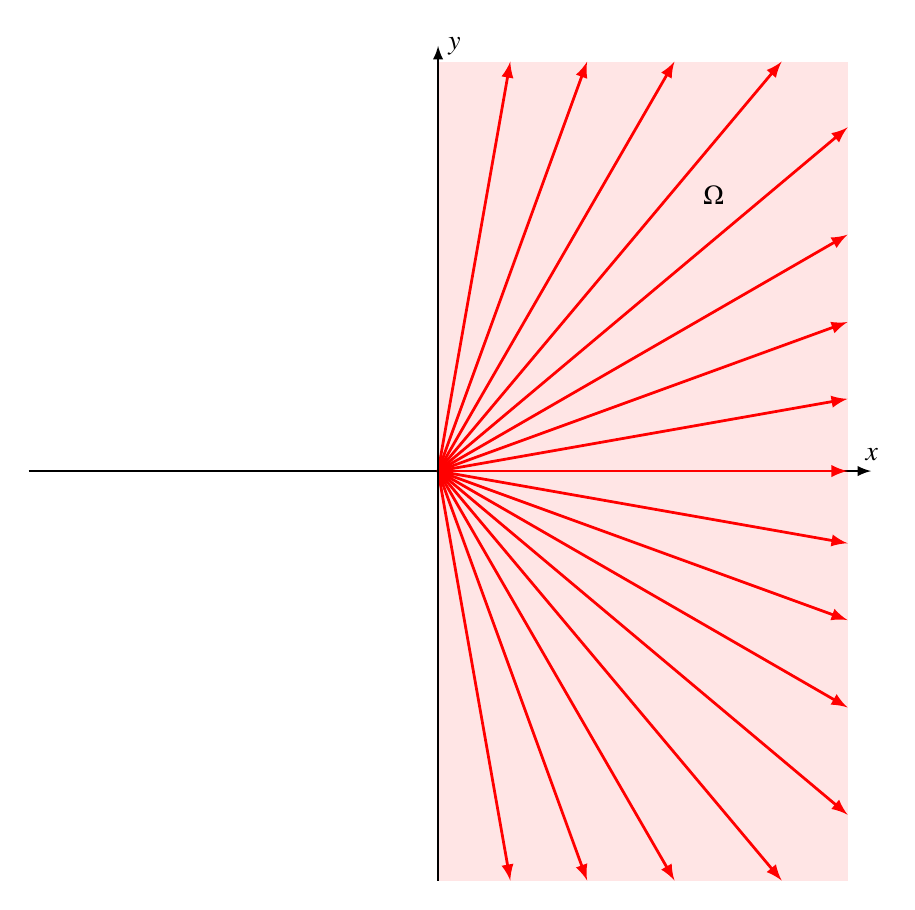
\begin{tikzpicture}[>=latex]

\fill[color=red!10] (0,-5.2) rectangle (5.2,5.2);

\draw[->,line width=0.7pt] (-5.2,0)--(5.5,0) coordinate[label={$x$}];

\foreach \a in {-40,-30,...,40}{
	\draw[->,line width=1pt,color=red] (0,0)--(5.2,{5.2*tan(\a)});
}
\foreach \a in {-80,-70,...,-50}{
	\draw[->,line width=1pt,color=red] (0,0)--({-5.2/tan(\a)},-5.2);
	\draw[->,line width=1pt,color=red] (0,0)--({-5.2/tan(\a)},5.2);
}

\node at (3.5,3.5) {$\Omega$};

\draw[->,line width=0.7pt] (0,-5.2)--(0,5.4) coordinate[label={right:$y$}];

\end{tikzpicture}
\end{document}

